\documentclass[aspectratio=43,9pt]{beamer}
%
\usepackage{graphicx,tikz}
\usepackage{enumerate}
\usepackage{setspace}
%
\usetheme{Boadilla}
%
\graphicspath{{./figures/}}
%
\let\Tiny=\tiny%			% to avoid warnings about font size
%\usepackage{lmodern}%		% alternative method to avoid these warnings
%
\catcode`~=11 % make LaTeX treat tilde (~) like a normal character
\newcommand{\urltilde}{\hbox{~}}
\catcode`~=13 % revert back to treating tilde (~) as an active character
%
% misc commands
\newcommand{\bm}[1]{\mathbf{#1}}
\newcommand{\bs}[1]{\boldsymbol{#1}}
\newenvironment{myitemize}[1]{\vspace{#1}\begin{itemize}\setlength\itemsep{#1}}{\end{itemize}}
%
% pgf markers
\usepgflibrary{plotmarks}
%
\setbeamertemplate{footline}
{
  \leavevmode%
  \hbox{%
  \begin{beamercolorbox}[wd=.8\paperwidth,ht=2.25ex,dp=1ex,left]{author in head/foot}%
    \usebeamerfont{author in head/foot}\hspace*{4em}\inserttitle
  \end{beamercolorbox}%
  \begin{beamercolorbox}[wd=.2\paperwidth,ht=2.25ex,dp=1ex,right]{author in head/foot}%
    \usebeamerfont{author in head/foot}\insertframenumber{} / \inserttotalframenumber\hspace*{1ex}
  \end{beamercolorbox}}%
  \vskip0pt%
}
%
\setbeamertemplate{navigation symbols}{}
%
\setbeamertemplate{frametitle}
{%
	\begin{minipage}{.9\paperwidth}
		\vspace*{1ex}%
		\flushright%
		%\bfseries
		\LARGE%
		\insertframetitle%
	\end{minipage}%
}
%
\setbeamertemplate{title page}{
	\begin{center}
		\vspace*{2ex}
		\usebeamercolor[fg]{frametitle}{%
			\Large%
			Numerical Techniques 2025--2026\\[2ex]
			%
			\LARGE%
			\inserttitle
		}\\[6ex]
		\usebeamercolor[fg]{normal text}{%
			Daan Degrauwe\\[1ex]
			\texttt{daan.degrauwe@meteo.be}\\[4ex]
			Postgraduate Studies in Weather and Climate Modeling\\[1ex]
			Ghent University
		}
	\end{center}
}
%
\newcommand{\ft}[2]{{\textstyle\frac{#1}{#2}}}
%
% increase space around equations
\makeatletter
\g@addto@macro\normalsize{%
	\setlength{\abovedisplayskip}{3ex}%
	\setlength{\belowdisplayskip}{3ex}%
	\setlength{\abovedisplayshortskip}{3ex}%
	\setlength{\belowdisplayshortskip}{3ex}%
}%
\makeatother
%

%
\title{5. Beyond the 1D advection equation}%
%
%%%%%%%%%%%%%%%%%%%%%%%%%%%%%%%%%%%%%%%%%%%%%%%%%%%%%%%%%%%%%%%%%%%%%%
%
\begin{document}
%
%%%%%%%%%%%%%%%%%%%%%%%%%%%%%%%%%%%%%%%%%%%%%%%%%%%%%%%%%%%%%%%%%%%%%%%%%%%%%%%%%%%%%%%%%%%%%%%%%%%%
%
\begin{frame}[plain]
	\titlepage
\end{frame}
%
%%%%%%%%%%%%%%%%%%%%%%%%%%%%%%%%%%%%%%%%%%%%%%%%%%%%%%%%%%%%%%%%%%%%%%
%
\begin{frame}
	%
	\frametitle{Content}
	\setstretch{1.5}
	%
	\begin{itemize}
		\item Systems of equations
			\begin{itemize}
				\item Shallow water equations
				\item Stability and dispersion relation
				\item Staggered grids
			\end{itemize}
		\item 2D problems
		\item Diffusion
		\item Nonlinearity
			\begin{itemize}
				\item Nonconstant advection speed and aliasing
				\item Burger's equation
				\item (Barotropic vorticity equation)
				\item Fibrillation
			\end{itemize}
	\end{itemize}
\end{frame}
%
%%%%%%%%%%%%%%%%%%%%%%%%%%%%%%%%%%%%%%%%%%%%%%%%%%%%%%%%%%%%%%%%%%%%%%
%
\begin{frame}
	\setstretch{1.5}
	\begin{itemize}
		\item {\bfseries Systems of equations}
		\item \textcolor{gray}{2D problems}
		\item \textcolor{gray}{Diffusion}
		\item \textcolor{gray}{Nonlinearity}
	\end{itemize}
\end{frame}
%
%%%%%%%%%%%%%%%%%%%%%%%%%%%%%%%%%%%%%%%%%%%%%%%%%%%%%%%%%%%%%%%%%%%%%%
%
\begin{frame}
	%
	\frametitle{Systems of equations}
	%
	\begin{itemize}
		\item We consider here systems with multiple dependent variables plus interaction between these variables (e.g. wind-pressure).\\[4ex]
			%
		\item Example: the linearized 1D shallow water equations (SWE) with unknowns $u$ and $h$:
			%
			\begin{align*}
				\frac{\partial u}{\partial t} + U \frac{\partial u}{\partial x} + g \frac{\partial h}{\partial x} &= 0 \\
				\frac{\partial h}{\partial t} + U \frac{\partial h}{\partial x} + H \frac{\partial u}{\partial x} &= 0
			\end{align*}
			%
			with $U$ and $H$ constants.
			%
			\par\vspace*{2ex}
			These equations are used very often to study numerical schemes.
			%
	\end{itemize}
	%
\end{frame}
%
%%%%%%%%%%%%%%%%%%%%%%%%%%%%%%%%%%%%%%%%%%%%%%%%%%%%%%%%%%%%%%%%%%%%%%
%
\begin{frame}
	%
	\frametitle{Systems of equations}
	%
	\begin{itemize}
		\item In matrix notation:
			%
			\begin{equation*}
				\frac{\partial \bm v}{\partial t}+\bm C\frac{\partial \bm v}{\partial x}=\bm 0
			\end{equation*}
			%
			where $\bm v$ is a vector containing the unknown fields
			%
			\begin{equation*}
				\bm v=\left(\begin{array}{c}u\\h\end{array}\right)
			\end{equation*}
			%
			and $\bf C$ is a $2\times2$ matrix:
			%
			\begin{equation*}
				\bm C=\left(\begin{array}{cc}U & g\\H &U\end{array}\right)
			\end{equation*}
			%
	\end{itemize}
	%
\end{frame}
%
%%%%%%%%%%%%%%%%%%%%%%%%%%%%%%%%%%%%%%%%%%%%%%%%%%%%%%%%%%%%%%%%%%%%%%
%
\begin{frame}
	%
	\frametitle{Systems of equations: stability}
	%
	\begin{itemize}
		\item Considering a harmonic shape for the solution,
			%
			\begin{equation*}
				\bm v_k = \left(\begin{array}{c} u_k \\ h_k\end{array}\right)e^{ikx},
			\end{equation*}
			%
			the time evolution can be written as
			%
			\begin{equation*}
				\bm v_k^{n+1}=\bm A_k \bm v_k^n
			\end{equation*}
			%
			with $\bm A_k$ the \emph{amplification matrix}.\vspace*{2ex}
			%
		\item A definition of stability (analogous to oscillation equation) is then:
			%
			\begin{equation*}
				\| {\bm v}_k^n \|  =  \| {\bm A}_k^n {\bm v}_k^0 \|  \le   \| {\bm v}_k^0 \|
			\end{equation*}
			%
	\end{itemize}
\end{frame}
%
%%%%%%%%%%%%%%%%%%%%%%%%%%%%%%%%%%%%%%%%%%%%%%%%%%%%%%%%%%%%%%%%%%%%%%
%
\begin{frame}
	%
	\frametitle{Systems of equations: stability}
	%
	\begin{itemize}
		\item Given the property that $\| {\bm A}_k^n \| \le \| {\bm A}_k \|^n$, a sufficient condition for stability is
			%
			\begin{equation*}
				\| {\bm A}_k \| \le 1
			\end{equation*}\vspace*{2ex}
			%
		\item This is a sufficient condition, but not a necessary one (see \emph{Durran} for an example).\vspace*{2ex}
			%
		\item Different matrix norms can be defined; the most common is the maximal eigenvalue:
			%
			\begin{equation*}
				\|\bm A\| = \max \left| \text{eig} (\bm A) \right|
			\end{equation*}
			%
	\end{itemize}
	%
\end{frame}
%
%%%%%%%%%%%%%%%%%%%%%%%%%%%%%%%%%%%%%%%%%%%%%%%%%%%%%%%%%%%%%%%%%%%%%%
%
\begin{frame}
	%
	\frametitle{Systems of equations: dispersion relation}
	%
	\begin{itemize}
		\item Like for the advection equation, a more powerful tool is the discrete dispersion relation.
		\item The dispersion relation is retrieved by assuming discretized harmonic waves (in space \emph{and} time) for $u$ and $h$
			%
			\begin{align*}
				u_j^n&=\hat u e^{i\left(k j \Delta x- \omega n \Delta t\right)}	\\
				h_j^n&=\hat h e^{i\left(k j \Delta x- \omega n \Delta t\right)}
			\end{align*}
			%
		\item For example, considering leapfrog time discretization and centered spatial differences, the SWE become
			%
			\begin{align*}
					\left(-\frac{\sin \omega \Delta t}{\Delta t} + U\frac{\sin k \Delta x}{\Delta x}\right) \hat u	+	g \frac{\sin k \Delta x}{\Delta x}\hat h	&	= 0	\\
					H \frac{\sin k \Delta x}{\Delta x}\hat u + \left(-\frac{\sin \omega \Delta t}{\Delta t} + U\frac{\sin k \Delta x}{\Delta x}\right) \hat h	&	= 0	\\
			\end{align*}
			%
			This homogeneous system only has a nontrivial (i.e. nonzero) solution if its determinant is zero.
	\end{itemize}
	%
\end{frame}
%
%%%%%%%%%%%%%%%%%%%%%%%%%%%%%%%%%%%%%%%%%%%%%%%%%%%%%%%%%%%%%%%%%%%%%%
%
\begin{frame}
	%
	\frametitle{Systems of equations: dispersion relation}
	%
	\begin{itemize}
		\item The determinant is zero if
			%
			\begin{equation*}
				\left(-\frac{\sin \omega \Delta t}{\Delta t} + U\frac{\sin k \Delta x}{\Delta x}\right)^2-gh\left(\frac{\sin k \Delta x}{\Delta x}\right)^2=0
			\end{equation*} 
			%
			or, with $c=\sqrt{gH}$
			%
			\begin{equation*}
				\sin\omega \Delta t=\frac{(U\pm c)\Delta t}{\Delta x}\sin k \Delta x
			\end{equation*}\vspace*{2ex}
			%
		\item This is the \emph{dispersion relation} of the SWE for this discretization. It should be compared with the exact dispersion relation for the SWE:
			%
			\begin{equation*}
				\omega=(U\pm c) k
			\end{equation*}
			%
	\end{itemize}
	%
\end{frame}
%
%%%%%%%%%%%%%%%%%%%%%%%%%%%%%%%%%%%%%%%%%%%%%%%%%%%%%%%%%%%%%%%%%%%%%%
%
\begin{frame}
	%
	\frametitle{Systems of equations: dispersion relation}
	%
	\begin{itemize}
		\item The $\pm$ symbol denotes that there are \emph{two} wave solutions (left-travelling and right-travelling), each with their own speed. In the atmosphere, even more wave-types exist: Rossby-wave, inertia-gravity waves, sound waves.\vspace*{2ex}
			%
		\item Note that the stability condition can be derived from the dispersion analysis, by requiring that $\omega$ is real:
			%
			\begin{equation*}
				\left |\frac{(U\pm c)\Delta t}{\Delta x} \right| \leq 1
			\end{equation*}
			%
	\end{itemize}
	%
\end{frame}
%
%%%%%%%%%%%%%%%%%%%%%%%%%%%%%%%%%%%%%%%%%%%%%%%%%%%%%%%%%%%%%%%%%%%%%%
%
\begin{frame}
	%
	\frametitle{Systems of equations: Staggering}
	%
	\begin{itemize}
		\item It is not strictly necessary to define all dependent variables in the same gridpoints.\vspace*{2ex}
			%
		\item E.g. for the linearized 1D shallow water equations you can define $u$ and $h$ at different gridpoints:
			%
			\par\vspace*{1ex}
			Not staggered:
			%
			\begin{center}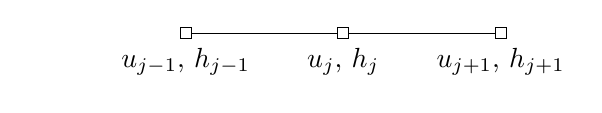
\begin{tikzpicture}[fill=white,>=latex]
				\draw (-2,0);
				\draw (0,0) -- (4,0);
				\draw plot[mark=square*] (0,0) node[below=2pt] {$u_{j-1}$, $h_{j-1}$} ;
				\draw plot[mark=square*] (2,0) node[below=2pt] {$u_{j}$, $h_{j}$};
				\draw plot[mark=square*] (4,0) node[below=2pt] {$u_{j+1}$, $h_{j+1}$};
			\end{tikzpicture}\end{center}
			%
			\vspace*{1ex}
			%
			Staggered:
			\begin{center}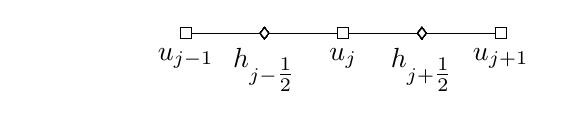
\begin{tikzpicture}[fill=white,>=latex]
				\draw (-2,0);
				\draw (0,0) -- (4,0);
				\draw plot[mark=square*] (0,0) node[below=2pt] {$u_{j-1}$} ;
				\draw plot[mark=diamond*] (1,0) node[below=2pt] {$h_{j-\ft12}$} ;
				\draw plot[mark=square*] (2,0) node[below=2pt] {$u_{j}$};
				\draw plot[mark=diamond*] (3,0) node[below=2pt] {$h_{j+\ft12}$};
				\draw plot[mark=square*] (4,0) node[below=2pt] {$u_{j+1}$};
			\end{tikzpicture}\end{center}\vspace*{2ex}
			%
		\item Advantage: spatial derivatives are calculated over a smaller grid distance (hence more accurate):
			%
			\begin{equation*}
				\left.\frac{\partial h}{\partial x}\right|_j\approx\frac{h_{j+\ft12}-h_{j-\ft12}}{\Delta x}
			\end{equation*}
			%
	\end{itemize}
	%
\end{frame}
%
%%%%%%%%%%%%%%%%%%%%%%%%%%%%%%%%%%%%%%%%%%%%%%%%%%%%%%%%%%%%%%%%%%%%%%
%
\begin{frame}
	%
	\frametitle{Systems of equations: Staggering}
	%
	\begin{itemize}
		\item Staggering solves the problem of negative groupspeeds of the shortest waves\vspace*{2ex}
			%
		\item In more spatial dimensions, the \emph{Arakawa C grid} is quite popular. Velocities are offset w.r.t. other variables (pressure, temperature, \ldots)\vspace*{2ex}
			%
			\begin{center}
				\footnotesize
				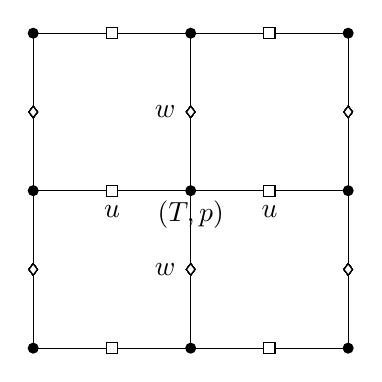
\begin{tikzpicture}[>=latex,x=1cm,y=1cm]
					\draw (0,0) -- +(2,0) -- +(4,0);
					\draw (0,2) -- +(2,0) -- +(4,0);
					\draw (0,4) -- +(2,0) -- +(4,0);
					\draw (0,0) -- +(0,2) -- +(0,4);
					\draw (2,0) -- +(0,2) -- +(0,4);
					\draw (4,0) -- +(0,2) -- +(0,4);
					%			
					\begin{scope}[fill=black]
						\fill (0,0) circle (2pt); \fill (2,0) circle (2pt); \fill (4,0) circle (2pt);
						\fill (0,2) circle (2pt);
						\fill (2,2) circle (2pt) node [below] {$(T,p)$};
						\fill (4,2) circle (2pt);
						\fill (0,4) circle (2pt); \fill (2,4) circle (2pt); \fill (4,4) circle (2pt);
					\end{scope}
					%
					\begin{scope}[mark=square*,fill=white]
						\draw plot (1,0); \draw plot (3,0);
						\draw plot (1,2) node [below=2pt] {$u$}; \draw plot (3,2) node [below=2pt] {$u$};
						\draw plot (1,4); \draw plot (3,4);
					\end{scope}
					%
					\begin{scope}[mark=diamond*,fill=white]
						\draw plot (0,1); \draw plot (0,3);
						\draw plot (2,1) node [left=2pt] {$w$}; \draw plot (2,3) node [left=2pt] {$w$};
						\draw plot (4,1); \draw plot (4,3);
					\end{scope}
				\end{tikzpicture}
			\end{center}\vspace*{2ex}
			%
		\item Interested? -- go for the student's project!
			%
	\end{itemize}
	%
\end{frame}
%
%%%%%%%%%%%%%%%%%%%%%%%%%%%%%%%%%%%%%%%%%%%%%%%%%%%%%%%%%%%%%%%%%%%%%%
%
\begin{frame}
	\setstretch{1.5}
	\begin{itemize}
		\item \textcolor{gray}{Systems of equations}
		\item {\bfseries 2D problems}
		\item \textcolor{gray}{Diffusion}
		\item \textcolor{gray}{Nonlinearity}
	\end{itemize}
\end{frame}
%
%%%%%%%%%%%%%%%%%%%%%%%%%%%%%%%%%%%%%%%%%%%%%%%%%%%%%%%%%%%%%%%%%%%%%%
%
\begin{frame}
	%
	\frametitle{More than two independent variables}
	%
	\begin{itemize}
		\item Example: the 2D advection equation
			%
			\begin{equation*}
				\frac{\partial \psi}{\partial t}+U\frac{\partial \psi}{\partial x}+V\frac{\partial \psi}{\partial y}=0
			\end{equation*}
			%
		\item Stability analysis of a scheme by inserting the wave solution
			%
			\begin{equation*}
				\phi^j_{m,n}=e^{i(km\Delta x+\ell n \Delta y-\omega j \Delta t)}
			\end{equation*}
			%
			For the space-centered leapfrog scheme and $\Delta x =\Delta y=\Delta s$, this yields:
			%
			\begin{equation*}
				(|U|+|V|)\frac{\Delta t}{\Delta s} < 1
			\end{equation*}
			%
			or, if $C$ is the maximum speed in the domain,
			%
			\begin{equation*}
				C\frac{\Delta t}{\Delta s} < \frac{1}{\sqrt{2}}
			\end{equation*}
	\end{itemize}
	%
\end{frame}
%
%%%%%%%%%%%%%%%%%%%%%%%%%%%%%%%%%%%%%%%%%%%%%%%%%%%%%%%%%%%%%%%%%%%%%%
%
\begin{frame}
	%
	\frametitle{More than two independent variables}
	%
	\begin{itemize}
		\item Reason for this more restrictive stability condition:
			%
			\begin{center}
				\scalebox{.6}{\small% GNUPLOT: LaTeX picture with Postscript
\begingroup
  \makeatletter
  \providecommand\color[2][]{%
    \GenericError{(gnuplot) \space\space\space\@spaces}{%
      Package color not loaded in conjunction with
      terminal option `colourtext'%
    }{See the gnuplot documentation for explanation.%
    }{Either use 'blacktext' in gnuplot or load the package
      color.sty in LaTeX.}%
    \renewcommand\color[2][]{}%
  }%
  \providecommand\includegraphics[2][]{%
    \GenericError{(gnuplot) \space\space\space\@spaces}{%
      Package graphicx or graphics not loaded%
    }{See the gnuplot documentation for explanation.%
    }{The gnuplot epslatex terminal needs graphicx.sty or graphics.sty.}%
    \renewcommand\includegraphics[2][]{}%
  }%
  \providecommand\rotatebox[2]{#2}%
  \@ifundefined{ifGPcolor}{%
    \newif\ifGPcolor
    \GPcolortrue
  }{}%
  \@ifundefined{ifGPblacktext}{%
    \newif\ifGPblacktext
    \GPblacktexttrue
  }{}%
  % define a \g@addto@macro without @ in the name:
  \let\gplgaddtomacro\g@addto@macro
  % define empty templates for all commands taking text:
  \gdef\gplbacktext{}%
  \gdef\gplfronttext{}%
  \makeatother
  \ifGPblacktext
    % no textcolor at all
    \def\colorrgb#1{}%
    \def\colorgray#1{}%
  \else
    % gray or color?
    \ifGPcolor
      \def\colorrgb#1{\color[rgb]{#1}}%
      \def\colorgray#1{\color[gray]{#1}}%
      \expandafter\def\csname LTw\endcsname{\color{white}}%
      \expandafter\def\csname LTb\endcsname{\color{black}}%
      \expandafter\def\csname LTa\endcsname{\color{black}}%
      \expandafter\def\csname LT0\endcsname{\color[rgb]{1,0,0}}%
      \expandafter\def\csname LT1\endcsname{\color[rgb]{0,1,0}}%
      \expandafter\def\csname LT2\endcsname{\color[rgb]{0,0,1}}%
      \expandafter\def\csname LT3\endcsname{\color[rgb]{1,0,1}}%
      \expandafter\def\csname LT4\endcsname{\color[rgb]{0,1,1}}%
      \expandafter\def\csname LT5\endcsname{\color[rgb]{1,1,0}}%
      \expandafter\def\csname LT6\endcsname{\color[rgb]{0,0,0}}%
      \expandafter\def\csname LT7\endcsname{\color[rgb]{1,0.3,0}}%
      \expandafter\def\csname LT8\endcsname{\color[rgb]{0.5,0.5,0.5}}%
    \else
      % gray
      \def\colorrgb#1{\color{black}}%
      \def\colorgray#1{\color[gray]{#1}}%
      \expandafter\def\csname LTw\endcsname{\color{white}}%
      \expandafter\def\csname LTb\endcsname{\color{black}}%
      \expandafter\def\csname LTa\endcsname{\color{black}}%
      \expandafter\def\csname LT0\endcsname{\color{black}}%
      \expandafter\def\csname LT1\endcsname{\color{black}}%
      \expandafter\def\csname LT2\endcsname{\color{black}}%
      \expandafter\def\csname LT3\endcsname{\color{black}}%
      \expandafter\def\csname LT4\endcsname{\color{black}}%
      \expandafter\def\csname LT5\endcsname{\color{black}}%
      \expandafter\def\csname LT6\endcsname{\color{black}}%
      \expandafter\def\csname LT7\endcsname{\color{black}}%
      \expandafter\def\csname LT8\endcsname{\color{black}}%
    \fi
  \fi
  \setlength{\unitlength}{0.0500bp}%
  \begin{picture}(4320.00,4320.00)%
    \gplgaddtomacro\gplbacktext{%
    }%
    \gplgaddtomacro\gplfronttext{%
      \colorrgb{0.00,0.00,0.00}%
      \put(2514,651){\makebox(0,0){\strut{}$2\Delta s$}}%
      \put(728,2528){\makebox(0,0)[l]{\strut{}$2\Delta s$}}%
      \put(2123,2059){\makebox(0,0)[l]{\strut{}$\sqrt{2}\Delta s$}}%
    }%
    \gplgaddtomacro\gplbacktext{%
    }%
    \gplgaddtomacro\gplfronttext{%
      \colorrgb{0.00,0.00,0.00}%
      \put(2514,651){\makebox(0,0){\strut{}$2\Delta s$}}%
      \put(728,2528){\makebox(0,0)[l]{\strut{}$2\Delta s$}}%
      \put(2123,2059){\makebox(0,0)[l]{\strut{}$\sqrt{2}\Delta s$}}%
    }%
    \gplbacktext
    \put(0,0){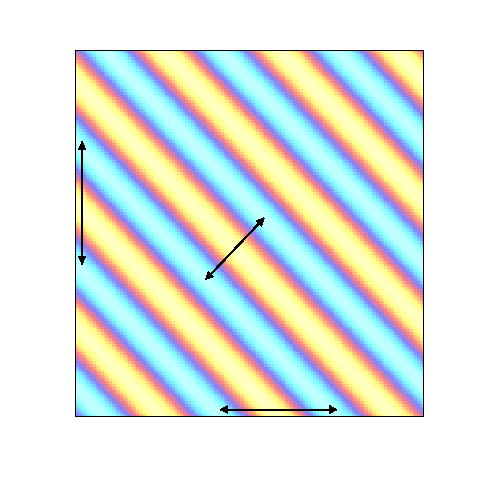
\includegraphics{2D}}%
    \gplfronttext
  \end{picture}%
\endgroup
}
			\end{center}
			%
			So a wave with wavelength $2\Delta s$ in the $x$-direction and $2\Delta s$ in the $y$-direction has a wavelength $\sqrt{2}\Delta s$ along the first bisector.
	\end{itemize}
	%
\end{frame}
%
%%%%%%%%%%%%%%%%%%%%%%%%%%%%%%%%%%%%%%%%%%%%%%%%%%%%%%%%%%%%%%%%%%%%%%
%
\begin{frame}
	\setstretch{1.5}
	\begin{itemize}
		\item \textcolor{gray}{Systems of equations}
		\item \textcolor{gray}{2D problems}
		\item {\bfseries Diffusion}
		\item \textcolor{gray}{Nonlinearity}
	\end{itemize}
\end{frame}
%
%%%%%%%%%%%%%%%%%%%%%%%%%%%%%%%%%%%%%%%%%%%%%%%%%%%%%%%%%%%%%%%%%%%%%%
%
\begin{frame}
	%
	\frametitle{Diffusion}
	%
	\begin{itemize}
		\item Diffusion is modeled with the following equation:
			%
			\begin{equation*}
				\frac{\partial \psi}{\partial t} = \frac{\partial}{\partial x} K \frac{\partial \psi}{\partial x}
			\end{equation*}
			%
			with $K > 0$.\vspace*{2ex}
			%
		\item Note that this is not a hyperbolic system (i.e. no wave solutions).\vspace*{2ex}
			%
		\item In NWP models such terms arise in the physics parameterisation (see \emph{Physical Meteorology: Surface and Turbulence}).
			%
	\end{itemize}
	%
\end{frame}
%
%%%%%%%%%%%%%%%%%%%%%%%%%%%%%%%%%%%%%%%%%%%%%%%%%%%%%%%%%%%%%%%%%%%%%%
%
\begin{frame}
	%
	\frametitle{Diffusion}
	%
	\begin{itemize}
		\item Diffusion flattens the peaks in a signal:
			%
			\begin{center}
				\scalebox{.7}{% GNUPLOT: LaTeX picture with Postscript
\begingroup
  \makeatletter
  \providecommand\color[2][]{%
    \GenericError{(gnuplot) \space\space\space\@spaces}{%
      Package color not loaded in conjunction with
      terminal option `colourtext'%
    }{See the gnuplot documentation for explanation.%
    }{Either use 'blacktext' in gnuplot or load the package
      color.sty in LaTeX.}%
    \renewcommand\color[2][]{}%
  }%
  \providecommand\includegraphics[2][]{%
    \GenericError{(gnuplot) \space\space\space\@spaces}{%
      Package graphicx or graphics not loaded%
    }{See the gnuplot documentation for explanation.%
    }{The gnuplot epslatex terminal needs graphicx.sty or graphics.sty.}%
    \renewcommand\includegraphics[2][]{}%
  }%
  \providecommand\rotatebox[2]{#2}%
  \@ifundefined{ifGPcolor}{%
    \newif\ifGPcolor
    \GPcolortrue
  }{}%
  \@ifundefined{ifGPblacktext}{%
    \newif\ifGPblacktext
    \GPblacktexttrue
  }{}%
  % define a \g@addto@macro without @ in the name:
  \let\gplgaddtomacro\g@addto@macro
  % define empty templates for all commands taking text:
  \gdef\gplbacktext{}%
  \gdef\gplfronttext{}%
  \makeatother
  \ifGPblacktext
    % no textcolor at all
    \def\colorrgb#1{}%
    \def\colorgray#1{}%
  \else
    % gray or color?
    \ifGPcolor
      \def\colorrgb#1{\color[rgb]{#1}}%
      \def\colorgray#1{\color[gray]{#1}}%
      \expandafter\def\csname LTw\endcsname{\color{white}}%
      \expandafter\def\csname LTb\endcsname{\color{black}}%
      \expandafter\def\csname LTa\endcsname{\color{black}}%
      \expandafter\def\csname LT0\endcsname{\color[rgb]{1,0,0}}%
      \expandafter\def\csname LT1\endcsname{\color[rgb]{0,1,0}}%
      \expandafter\def\csname LT2\endcsname{\color[rgb]{0,0,1}}%
      \expandafter\def\csname LT3\endcsname{\color[rgb]{1,0,1}}%
      \expandafter\def\csname LT4\endcsname{\color[rgb]{0,1,1}}%
      \expandafter\def\csname LT5\endcsname{\color[rgb]{1,1,0}}%
      \expandafter\def\csname LT6\endcsname{\color[rgb]{0,0,0}}%
      \expandafter\def\csname LT7\endcsname{\color[rgb]{1,0.3,0}}%
      \expandafter\def\csname LT8\endcsname{\color[rgb]{0.5,0.5,0.5}}%
    \else
      % gray
      \def\colorrgb#1{\color{black}}%
      \def\colorgray#1{\color[gray]{#1}}%
      \expandafter\def\csname LTw\endcsname{\color{white}}%
      \expandafter\def\csname LTb\endcsname{\color{black}}%
      \expandafter\def\csname LTa\endcsname{\color{black}}%
      \expandafter\def\csname LT0\endcsname{\color{black}}%
      \expandafter\def\csname LT1\endcsname{\color{black}}%
      \expandafter\def\csname LT2\endcsname{\color{black}}%
      \expandafter\def\csname LT3\endcsname{\color{black}}%
      \expandafter\def\csname LT4\endcsname{\color{black}}%
      \expandafter\def\csname LT5\endcsname{\color{black}}%
      \expandafter\def\csname LT6\endcsname{\color{black}}%
      \expandafter\def\csname LT7\endcsname{\color{black}}%
      \expandafter\def\csname LT8\endcsname{\color{black}}%
    \fi
  \fi
  \setlength{\unitlength}{0.0500bp}%
  \begin{picture}(8640.00,4320.00)%
    \gplgaddtomacro\gplbacktext{%
    }%
    \gplgaddtomacro\gplfronttext{%
      \colorrgb{0.00,0.00,0.00}%
      \put(1624,3311){\makebox(0,0)[l]{\strut{}$\frac{d^2\psi}{dx^2}<0$}}%
      \put(5702,2873){\makebox(0,0)[l]{\strut{}$\frac{d^2\psi}{dx^2}<0$}}%
      \put(3698,766){\makebox(0,0)[l]{\strut{}$\frac{d^2\psi}{dx^2}>0$}}%
      \put(6947,2397){\makebox(0,0)[r]{\strut{}$\frac{d^2\psi}{dx^2}>0$}}%
    }%
    \gplbacktext
    \put(0,0){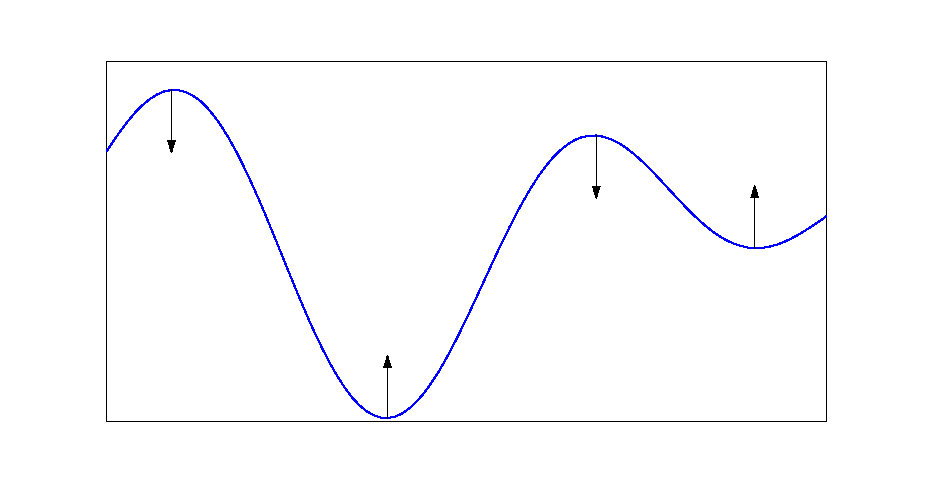
\includegraphics{diffusion}}%
    \gplfronttext
  \end{picture}%
\endgroup
}
			\end{center}
			%
		\item So it should be inherently stable\ldots
			%
	\end{itemize}
	%
\end{frame}
%
%%%%%%%%%%%%%%%%%%%%%%%%%%%%%%%%%%%%%%%%%%%%%%%%%%%%%%%%%%%%%%%%%%%%%%
%
\begin{frame}
	%
	\frametitle{Diffusion}
	%
	\begin{itemize}
		\item Let us discretize with a forward-time, centered-space scheme:
			%
			\begin{equation*}
				\frac{\phi^{n+1}_j - \phi^n_j}{\Delta t} = K\delta_x^2\phi^n_j
			\end{equation*}
			%
			where $\delta_x^2\phi_j=\frac{\phi_{j+1} - 2 \, \phi_j + \phi_{j-1}}{\Delta x^2}$
			%
		\item Von Neuman stability analysis shows that the amplification factor is
			%
			\begin{equation*}
				A_k = 1 - 2 \nu \left(
					1 - \cos k \Delta x
				\right)
			\end{equation*}
			%
			with
			%
			\begin{equation*}
				\nu = \frac{K \Delta t}{\Delta x^2}
			\end{equation*}
			%
			The scheme is stable provided $\left|A_k\right|^2\le 1$, i.e. if
			%
			\begin{equation*}
				0 < \nu \le \ft12
			\end{equation*}
			%
	\end{itemize}
	%
\end{frame}
%
%%%%%%%%%%%%%%%%%%%%%%%%%%%%%%%%%%%%%%%%%%%%%%%%%%%%%%%%%%%%%%%%%%%%%%
%
\begin{frame}
	%
	\frametitle{Diffusion}
	%
	\begin{itemize}
		\item Note that due to the form of $\nu = \frac{K \Delta t}{\Delta x^2}$ this scheme does not stay stable when $\Delta t, \Delta x \rightarrow 0$
	unless $\Delta t$ decreases much more rapidly than $\Delta x$!\vspace*{2ex}
			%
		\item This makes this scheme very inefficient at high resolutions!
		%
	\end{itemize}
	%
\end{frame}
%
%%%%%%%%%%%%%%%%%%%%%%%%%%%%%%%%%%%%%%%%%%%%%%%%%%%%%%%%%%%%%%%%%%%%%%
%
\begin{frame}
	%
	\frametitle{Diffusion}
	%
	\begin{itemize}
		\item With trapezium time differencing
		%
		\begin{equation*}
			\frac{\phi^{n+1} - \phi^n}{\Delta t} =\frac{K}{2}\left(\delta_x^2 \phi^{n+1}_j + \delta_x^2 \phi^n_j\right)
		\end{equation*}
		%
		the amplification factor becomes
		%
		\begin{equation*}
			A_k = \frac{1 - \nu \left( 1 - \cos k \Delta x \right)}	{1 + \nu \left( 1 - \cos k \Delta x \right)}
		\end{equation*}
		%
		So if $K > 0$ then  $| A_k | \le 1$ for	all $\Delta t$.
		%
	\end{itemize}
\end{frame}
%
%%%%%%%%%%%%%%%%%%%%%%%%%%%%%%%%%%%%%%%%%%%%%%%%%%%%%%%%%%%%%%%%%%%%%%
%
\begin{frame}
	%
	\frametitle{Diffusion}
	%
	\begin{itemize}
		\item However, one now has to solve a tridiagonal system (in 1D):
			%
			\begin{equation*}
				\left(\begin{array}{ccccc}
					\ddots\\
					\cdots & 1+\nu &-\nu/2 & 0 & \cdots \\
					\cdots & -\nu/2 & 1+\nu & -\nu/2 & \cdots \\
					\cdots & 0 & -\nu/2 & 1+\nu & \cdots \\
					&&&&\ddots
				\end{array}\right)\left(\begin{array}{c}\vdots \\ \phi_{j-1} \\ \phi_j \\ \phi_{j+1} \\ \vdots \end{array}\right)^{n+1}
					= \ldots
			\end{equation*}\vspace*{2ex}
			%
		\item So the question becomes, does the increase in the  time step $\Delta t$ outweigh the increase in computing cost for the solver?
			%
	\end{itemize}
	%
\end{frame}
%
%%%%%%%%%%%%%%%%%%%%%%%%%%%%%%%%%%%%%%%%%%%%%%%%%%%%%%%%%%%%%%%%%%%%%%
%
\begin{frame}
	\setstretch{1.5}
	\begin{itemize}
		\item \textcolor{gray}{Systems of equations}
		\item \textcolor{gray}{2D problems}
		\item \textcolor{gray}{Diffusion}
		\item {\bfseries Nonlinearity}
	\end{itemize}
\end{frame}
%
%%%%%%%%%%%%%%%%%%%%%%%%%%%%%%%%%%%%%%%%%%%%%%%%%%%%%%%%%%%%%%%%%%%%%%
%
\begin{frame}
	%
	\frametitle{Nonlinearity}
	%
	We will consider the following examples of nonlinear systems:\vspace*{4ex}
	%
	\begin{itemize}
		\item Variable advection speed and aliasing\vspace*{2ex}
		\item Burger's equation and shock development\vspace*{2ex}
		\item (The barotropic vorticity equation)\vspace*{2ex}
		\item Fibrillation due to nonlinear diffusion
	\end{itemize}
	%
\end{frame}
%
%%%%%%%%%%%%%%%%%%%%%%%%%%%%%%%%%%%%%%%%%%%%%%%%%%%%%%%%%%%%%%%%%%%%%%
%
\begin{frame}
	%
	\frametitle{Variable advection speed: aliasing}
	%
	\begin{itemize}
		\item We consider the 1D advection equation with variable wind $c(x)$,
			%
			\begin{equation*}
				\frac{\partial \psi}{\partial t} + c(x) \frac{\partial \psi}{\partial x} = 0
			\end{equation*}
			%
		\item Let us consider a discretization on $N$ gridpoints on a domain $[0,2\pi)$. Suppose that the wind $c(x)$ and the initial state $\psi(t=0)$ are composed of waves with wavenumbers $0$, $N/4$ and $N/2$ (i.e. wavelengths $\infty$, $4\Delta x$ and $2\Delta x$):
			%
			\begin{align*}
				c(x_j) &= c_0 + (c_r+ic_i) e^{i \pi j/2} + (c_r-ic_i) e^{-i \pi j/2} + c_n e^{i \pi j} \\
				\phi(x_j) &= a_0 + (a_r+ia_i) e^{i \pi j/2} + (a_r-ia_i) e^{-i \pi j/2} + a_n e^{i \pi j}
			\end{align*}
			%
		\item We may expect aliasing, e.g.
			%
			\begin{equation*}
				e^{i \pi j /2} e^{i \pi j} = e^{i 3 \pi j /2} = e^{- i \pi j/2}
			\end{equation*}
			%
	\end{itemize}
\end{frame}
%
%%%%%%%%%%%%%%%%%%%%%%%%%%%%%%%%%%%%%%%%%%%%%%%%%%%%%%%%%%%%%%%%%%%%%%
%
\begin{frame}
	%
	\frametitle{Variable advection speed: aliasing}
	%
	\begin{itemize}
		\item One can show that with centered spatial differences, the exact time evolution of the spectral coefficients $a_0$, $a_r$, $a_i$, $a_n$ is given by:
			%
			\begin{align*}
				\frac{d a_0}{dt} &= 2 \frac{a_i c_r - a_r c_i}{\Delta x}	&
				\frac{d a_n}{dt} &= 2 \frac{a_i c_r + a_r c_i}{\Delta x}	\\
				\frac{d a_r}{dt} &= a_i \frac{c_n + c_0}{\Delta x}	&
				\frac{d a_i}{dt} &= a_r \frac{c_n - c_0}{\Delta x}
			\end{align*}
			%
		\item Eliminating $a_i$, we find for the time evolution of $a_r$:
			%
			\begin{equation*}
				\frac{d^2 a_r}{dt^2} = \frac{c_n^2 - c_0^2}{\Delta x^2} a_r
			\end{equation*}
			%
			which has an exponential solution!
			%
		\item So with this discretization, we get an instability if $c_n > c_0$, regardless of the time discretization!.
			%
		\item This growth is unphysical since the solution is bounded by the maximum value of $\psi$.
			%
	\end{itemize}
	%	
\end{frame}
%
%%%%%%%%%%%%%%%%%%%%%%%%%%%%%%%%%%%%%%%%%%%%%%%%%%%%%%%%%%%%%%%%%%%%%%
%
\begin{frame}
	%
	\frametitle{Burger's equation}
	%
	\begin{itemize}
		\item Another example of nonlinear instability is Burger's equation:
			%
			\begin{equation*}
			 \frac{\partial \psi}{\partial t} + \psi \frac{\partial \psi}{\partial x} = 0
			\end{equation*}
			%
		\item If the initial condition is $\psi(x,t=0)=f(x)$, then the solution can be written implicitly as
			%
			\begin{equation*}
				\psi(x,t) = f ( x - \psi(x,t) t)
			\end{equation*}
			%
			So $\psi$ is constant along the so-called \emph{characteristic curves} in the $(x,t)$ plane:
			%
			\begin{equation*}
				x - \psi(x,t) t = cst.
			\end{equation*}
			%
	\end{itemize}
	%
\end{frame}
%
%%%%%%%%%%%%%%%%%%%%%%%%%%%%%%%%%%%%%%%%%%%%%%%%%%%%%%%%%%%%%%%%%%%%%%
%
\begin{frame}
	%
	\frametitle{Burger's equation}
	%
	\begin{itemize}
		\item We can expect some problems: consider a sine-like initial condition:
			%
			\begin{center}
				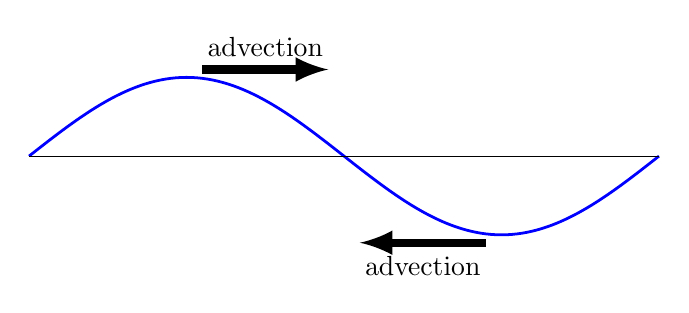
\begin{tikzpicture}[>=latex,x=2cm]
					\draw[blue,line width=1pt] (0,0) sin (1,1) cos (2,0) sin (3,-1) cos (4,0);
					\draw (0,0) -- (4,0);
					\draw[line width=3pt,->] (1.1,1.1) -- +(0.8,0) node [pos=0.5,above] {advection};
					\draw[line width=3pt,->] (2.9,-1.1) -- +(-0.8,0) node [pos=0.5,below] {advection};
				\end{tikzpicture}
			\end{center}
			%
		\item Eventually, a shock will develop.
			%
	\end{itemize}
	%
\end{frame}
%
%%%%%%%%%%%%%%%%%%%%%%%%%%%%%%%%%%%%%%%%%%%%%%%%%%%%%%%%%%%%%%%%%%%%%%
%
\begin{frame}
	%
	\frametitle{Burger's equation}
	%
	\begin{itemize}
		\item One can show that the $\ell_2$-norm of the exact solution over a periodic domain $[0,1]$ is conserved (so the shock will remain limited in the exact solution):
			%
			\begin{equation*}
				\frac{\partial}{\partial t}\int_0^1 \psi(x,t)^2 dx=0
			\end{equation*}
			%
		\item However, when discretizing Burger's equation as
			%
			\begin{equation*}
				\frac{ d\phi_j}{d t}+\phi_j\left(\frac{\phi_{j+1}-\phi_{j-1}}{2 \Delta x}\right)=0
			\end{equation*}
			%
			the $\ell_2$-norm is not conserved:
			%
			\begin{equation*}
				\frac{d }{dt}\sum_j \phi_j^2=\sum_j \phi_j\phi_{j+1}\left(\frac{\phi_{j+1}-\phi_j}{\Delta x}\right)
			\end{equation*}
			%
	\end{itemize}
	%
\end{frame}
%
%%%%%%%%%%%%%%%%%%%%%%%%%%%%%%%%%%%%%%%%%%%%%%%%%%%%%%%%%%%%%%%%%%%%%%
%
\begin{frame}
	%
	\frametitle{Burger's equation}
	%
	\begin{itemize}
		\item We can try a different shape (`flux-shape') of Burger's equation:
			%
			\begin{equation*}
				\frac{\partial \psi}{\partial t} + \frac{1}{2} \frac{\partial \psi^2}{\partial x} = 0
			\end{equation*}
			%
			which is discretized as:
			%
			\begin{equation*}
				\frac{d \phi_j}{dt}  + \ft12 \frac{\phi_{j+1}^2 - \phi_{j-1}^2}{2 \Delta x} = 0
			\end{equation*}
			%
		\item This leads to
			%
			\begin{equation*}
				\frac{d}{dt} \sum_j \phi_j^2 =-\ft12	\sum_j \phi_j \phi_{j+1}\frac{\phi_{j+1} - \phi_j}{\Delta x}	\ne 0
			\end{equation*}
			%
			so it doesn't conserve the norm either.
			%
	\end{itemize}
	%
\end{frame}
%
%%%%%%%%%%%%%%%%%%%%%%%%%%%%%%%%%%%%%%%%%%%%%%%%%%%%%%%%%%%%%%%%%%%%%%
%
\begin{frame}
	%
	\frametitle{Burger's equation}
	%
	\begin{itemize}
		\item It's possible to make a combination of these two alternatives:
			%
			\begin{equation*}
				\frac{d \phi_j}{dt}  + \ft23 \frac{\phi_{j+1}^2 - \phi_{j-1}^2}{2 \Delta x}  +\ft13 \frac{\phi_{j+1} - \phi_{j-1}}{2 \Delta x} \phi_j = 0
			\end{equation*}
			%
		\item The contributions of both schemes to the norm evolution will cancel out, so this scheme conserves the norm
			%
			\begin{equation*}
				\frac{d}{dt} \sum_j \phi_j^2 = 0
			\end{equation*}
			%
			and doesn't blow up.
			%
	\end{itemize}
	%
\end{frame}
%
%%%%%%%%%%%%%%%%%%%%%%%%%%%%%%%%%%%%%%%%%%%%%%%%%%%%%%%%%%%%%%%%%%%%%%
%
\begin{frame}
	%
	\frametitle{Burger's equation}
	%
	\begin{itemize}
		\item In reality there is always some diffusion
			%
			\begin{equation*}
				\frac{\partial \psi}{\partial t} + \psi \frac{\partial \psi}{\partial x} = \nu \frac{\partial^2 \psi}{\partial x^2}
			\end{equation*}\vspace*{2ex}
			%
		\item Then the true solution never develops a shock. However, if discretized with the advective form, a scheme can develop a shock for sufficiently small values of $\nu$.\vspace*{2ex}
			%
		\item This is another reason for introducing some dosis of (artificial) numerical diffusion.
			%
	\end{itemize}
	%
\end{frame}
%
%%%%%%%%%%%%%%%%%%%%%%%%%%%%%%%%%%%%%%%%%%%%%%%%%%%%%%%%%%%%%%%%%%%%%%
%
\begin{frame}
	%
	\frametitle{Barotropic vorticity equation}
	%
	\begin{itemize}
		\item The barotropic vorticity equation (see \emph{Dynamic Meteorology}) is written as:
			%
			\begin{equation*}
				\frac{\partial \zeta}{\partial t} + \bm u \cdot \nabla \zeta = 0
			\end{equation*}
			%
			with $\bm u$ the geostrophic wind\vspace*{-1mm}
			%
			\begin{equation*}
				\bm u = \bm k \times \nabla \psi
			\end{equation*}
			%
			and the vorticity\vspace*{-1mm}
			%
			\begin{equation*}
				\zeta = \bm k \cdot \nabla \times \bm u =\nabla^2\psi
			\end{equation*}
			%
		\item Although this a nonlinear equation, one can show that there is no \emph{net} energy transfer between scales (the average wavenumber is conserved).
			%
		\item Here too, a clever discretization satisfies this conservation constraint, and allows to suppress the nonlinear instability.
			%
			\par\vspace*{2ex}
			-- see student's projects.
			%
	\end{itemize}
	%
\end{frame}
%
%%%%%%%%%%%%%%%%%%%%%%%%%%%%%%%%%%%%%%%%%%%%%%%%%%%%%%%%%%%%%%%%%%%%%%
%
\begin{frame}
	%
	\frametitle{Fibrillation}
	%
	\begin{itemize}
		\item Nonlinear instabilities also have an effect in the diffusion equation.\vspace*{2ex}
		\item This can be studied in its most easy form in the damping equations,
			%
			\begin{equation*}
				\frac{\partial \psi}{\partial t} = - \left( K \psi^P \right) \psi + S
			\end{equation*}
			%
			with $K$ a constant representing the amount of damping, and $P$ the degree of nonlinearity. $S$ is an external forcing.\vspace*{2ex}
			%
		\item This equation has been studied by Kalnay and Kanamitsu (1988) (Mon. Wea. Rev., 116, 1945-1958) and is considered as the reference test for diffusion schemes in atmospheric models.
	\end{itemize}
	%
\end{frame}
%
%%%%%%%%%%%%%%%%%%%%%%%%%%%%%%%%%%%%%%%%%%%%%%%%%%%%%%%%%%%%%%%%%%%%%%
%
\begin{frame}
	%
	\frametitle{Fibrillation}
	%
	\begin{itemize}
		\item The equation is discretized as
			%
			\begin{equation*}
				\frac{\phi_{n+1} - \phi_n}{\Delta t} = - K \phi_n^P \left[ \gamma \phi_{n+1} + (1-\gamma) \phi_n \right] + S_n
			\end{equation*}
			%
			with $\Delta t =1$, and the forcing is set to
			%
			\begin{equation*}
				S_n = 1 + \sin \left (\frac{2 \pi n}{20}\right)
			\end{equation*}
			%
			(think of this as a radiative forcing).
			%
		\item The parameter $\gamma$ determines the degree of implicitness ($\gamma=0.5$ is trapezium-like).
			%
	\end{itemize}
	%
\end{frame}
%
%%%%%%%%%%%%%%%%%%%%%%%%%%%%%%%%%%%%%%%%%%%%%%%%%%%%%%%%%%%%%%%%%%%%%%
%
\begin{frame}
	%
	\frametitle{Fibrillation}
	%
	With $K=10$ and $P=2$ and with $\gamma=1/2$, we get following results:
	%
	\begin{center}
		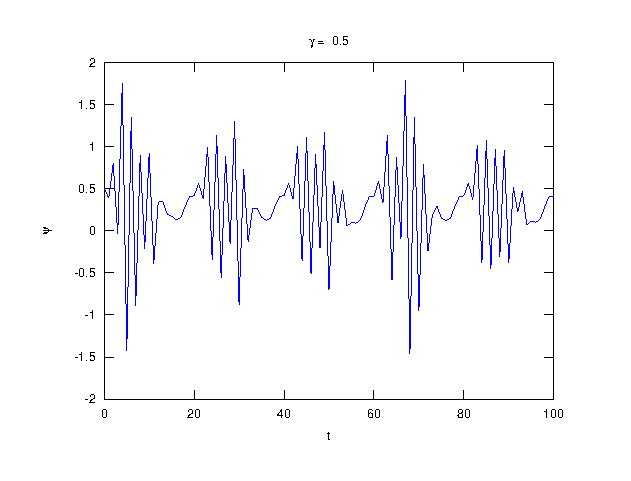
\includegraphics[scale=0.8]{fib_a}
	\end{center}
	%
	\par
	Similar behavior is also encountered in a 3D NWP model.
	%
\end{frame}
%
%%%%%%%%%%%%%%%%%%%%%%%%%%%%%%%%%%%%%%%%%%%%%%%%%%%%%%%%%%%%%%%%%%%%%%
%
\begin{frame}
	%
	\frametitle{Fibrillation}
	%
	\begin{itemize}
		\item We see nonsensical oscillations in time.\vspace*{1ex}
		\item These are not unstabilities in the sense that the model blows up.\vspace*{1ex}
		\item They can not be understood by linear stability analysis.\vspace*{1ex}
		\item Contrary to Burger's equations, we do not know the exact solution, so we can not analyse it on paper.\vspace*{1ex}
		\item However, they should be eliminated: invent schemes and choose the most convenient one (see \emph{Kalnay and Kanamitsu}).\\[1ex]
			A popular solution is \emph{over-implicitness} (i.e. $\gamma>1$).
	\end{itemize}
	%
\end{frame}
%
%%%%%%%%%%%%%%%%%%%%%%%%%%%%%%%%%%%%%%%%%%%%%%%%%%%%%%%%%%%%%%%%%%%%%%
%
\begin{frame}
	%
	\frametitle{Fibrillation}
	%
	\begin{center}
		\only<1>{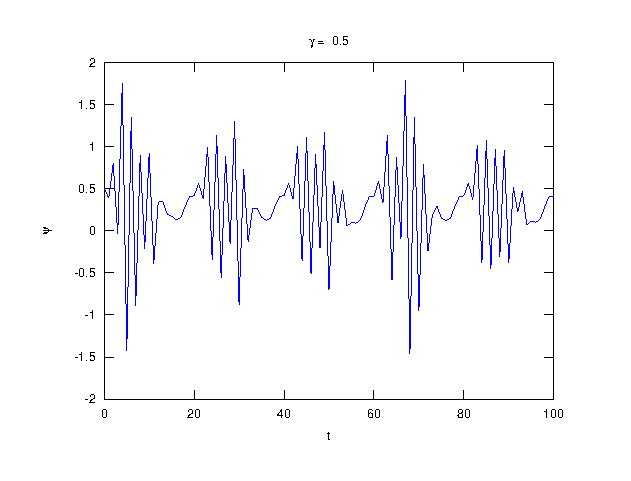
\includegraphics[scale=0.9]{fib_a}}%
		\only<2>{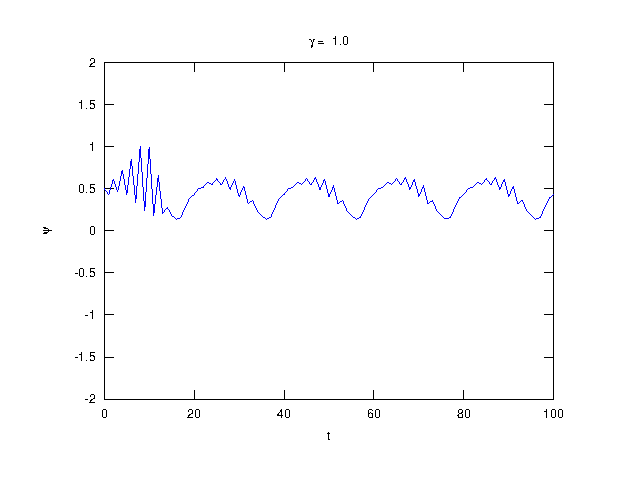
\includegraphics[scale=0.9]{fib_b}}%
		\only<3>{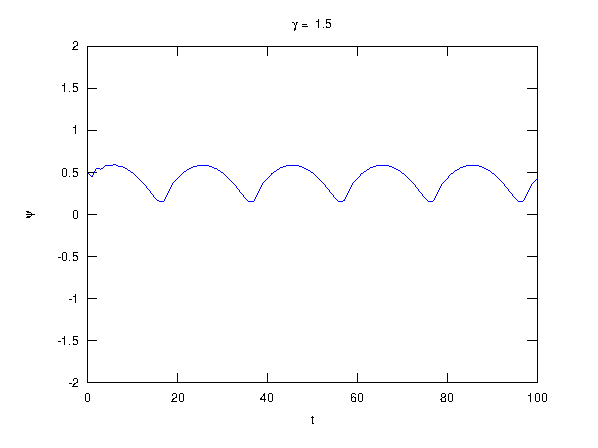
\includegraphics[scale=0.9]{fib_c}}%
	\end{center}
	%
\end{frame}
%
%%%%%%%%%%%%%%%%%%%%%%%%%%%%%%%%%%%%%%%%%%%%%%%%%%%%%%%%%%%%%%%%%%%%%%
%
\begin{frame}
	%
	\frametitle{Some overview remarks}
	%
	\begin{itemize}
		\item Try to see links with other lessons and other courses:\vspace*{1ex}
			\begin{itemize}
				\item Stability and dispersion for systems of equations is (almost) the same as for scalar equations, with matrices replacing scalars.\vspace*{1ex}
				\item Aliasing is closely related to nonlinearity\vspace*{1ex}
				\item Barotropic vorticity equation $\Leftarrow$ \emph{Dynamic Meteorology}\vspace*{1ex}
				\item Diffusion equation $\Leftarrow$ \emph{Physical Meteorology}
			\end{itemize}\vspace*{2ex}
		\item Methodology is more important than algebra! Think in terms of waves\ldots\vspace*{2ex}
		\item This course is about \emph{surprising} results due to numerical discretization.\vspace*{1ex}
			\begin{itemize}
				\item stability in 2D is more stringent than in 1D\vspace*{1ex}
				\item even for the diffusion equation, unstable behaviour may occur\vspace*{1ex}
				\item nonlinearity may lead to instability, even with supposedly stable schemes.\vspace*{1ex}
				\item \ldots\vspace*{2ex}
			\end{itemize}
		\item If something is unclear, you should pick the corresponding student's project!
	\end{itemize}
\end{frame}
%
%%%%%%%%%%%%%%%%%%%%%%%%%%%%%%%%%%%%%%%%%%%%%%%%%%%%%%%%%%%%%%%%%%%%%%
%
\end{document}
